\begin{figure*}[!t]
  \centering
  \small
  \begin{minipage}[t]{0.48\textwidth}
    \centering
    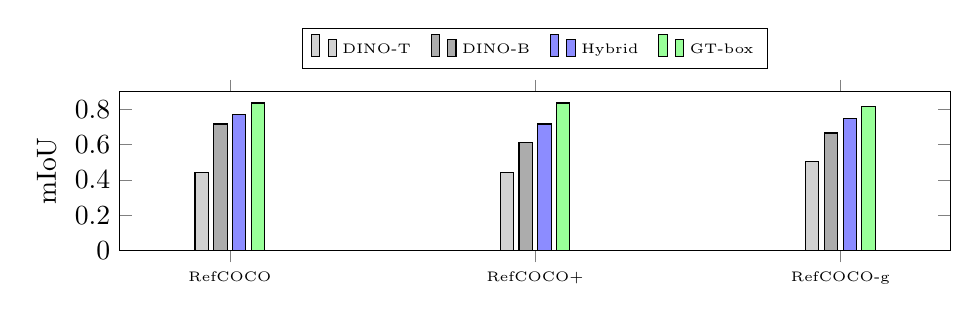
\begin{tikzpicture}
      \begin{axis}[
        width=\linewidth, height=3.6cm, ybar, bar width=4.8pt,
        ymin=0, ymax=0.90, ylabel={mIoU},
        symbolic x coords={RefCOCO,RefCOCO+,RefCOCO-g},
        xtick=data, xticklabel style={font=\tiny},
        enlarge x limits=0.18,
        legend style={
          font=\tiny,
          at={(0.5,1.14)},
          anchor=south,
          legend columns=4,
          /tikz/every even column/.append style={column sep=0.18cm}
        },
      ]
        \addplot[fill=gray!35] coordinates {(RefCOCO,0.441) (RefCOCO+,0.440) (RefCOCO-g,0.503)};
        \addplot[fill=gray!65] coordinates {(RefCOCO,0.717) (RefCOCO+,0.612) (RefCOCO-g,0.666)};
        \addplot[fill=blue!45] coordinates {(RefCOCO,0.772) (RefCOCO+,0.717) (RefCOCO-g,0.746)};
        \addplot[fill=green!40] coordinates {(RefCOCO,0.836) (RefCOCO+,0.836) (RefCOCO-g,0.815)};
        \legend{DINO-T,DINO-B,Hybrid,GT-box}
      \end{axis}
    \end{tikzpicture}
    \par\vspace{0.15em}(a) Main mIoU across validation splits
  \end{minipage}\hfill
  \begin{minipage}[t]{0.48\textwidth}
    \centering
    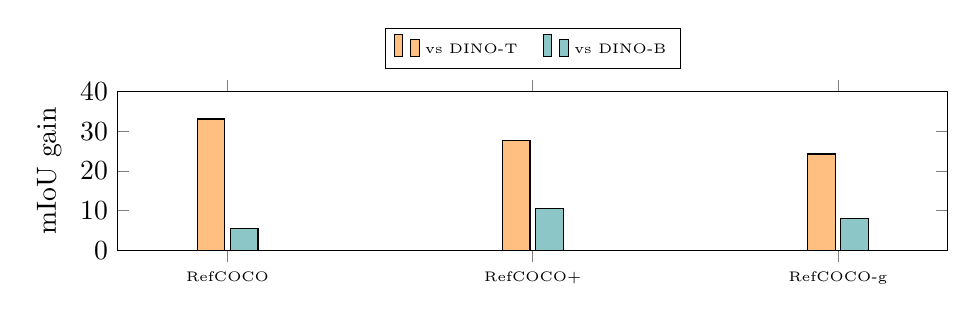
\begin{tikzpicture}
      \begin{axis}[
        width=\linewidth, height=3.6cm, ybar, bar width=10pt,
        ymin=0, ymax=40, ylabel={mIoU gain},
        symbolic x coords={RefCOCO,RefCOCO+,RefCOCO-g},
        xtick=data, xticklabel style={font=\tiny},
        enlarge x limits=0.18,
        legend style={
          font=\tiny,
          at={(0.5,1.14)},
          anchor=south,
          legend columns=2,
          /tikz/every even column/.append style={column sep=0.25cm}
        },
      ]
        \addplot[fill=orange!50] coordinates {(RefCOCO,33.1) (RefCOCO+,27.7) (RefCOCO-g,24.3)};
        \addplot[fill=teal!45] coordinates {(RefCOCO,5.5) (RefCOCO+,10.5) (RefCOCO-g,8.0)};
        \legend{vs DINO-T,vs DINO-B}
      \end{axis}
    \end{tikzpicture}
    \par\vspace{0.15em}(b) Hybrid gain over matched baselines
  \end{minipage}

  \vspace{0.55em}

  \begin{minipage}[t]{0.48\textwidth}
    \centering
    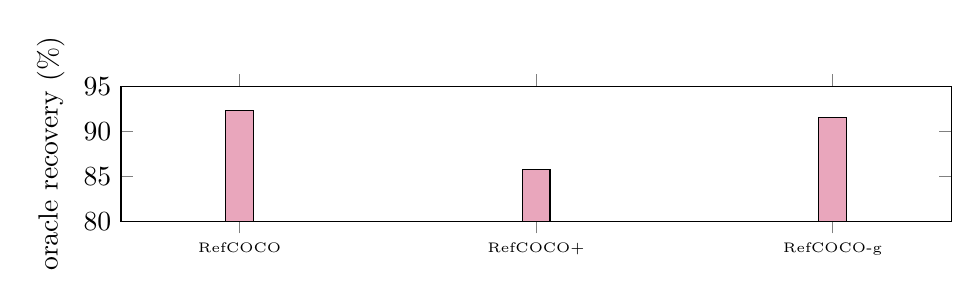
\begin{tikzpicture}
      \begin{axis}[
        width=\linewidth, height=3.3cm, ybar, bar width=10pt,
        ymin=80, ymax=95, ylabel={oracle recovery (\%)},
        symbolic x coords={RefCOCO,RefCOCO+,RefCOCO-g},
        xtick=data, xticklabel style={font=\tiny},
        enlarge x limits=0.2,
      ]
        \addplot[fill=purple!35] coordinates {(RefCOCO,92.3) (RefCOCO+,85.8) (RefCOCO-g,91.5)};
      \end{axis}
    \end{tikzpicture}
    \par\vspace{0.15em}(c) Hybrid as a percentage of GT-box oracle
  \end{minipage}\hfill
  \begin{minipage}[t]{0.48\textwidth}
    \centering
    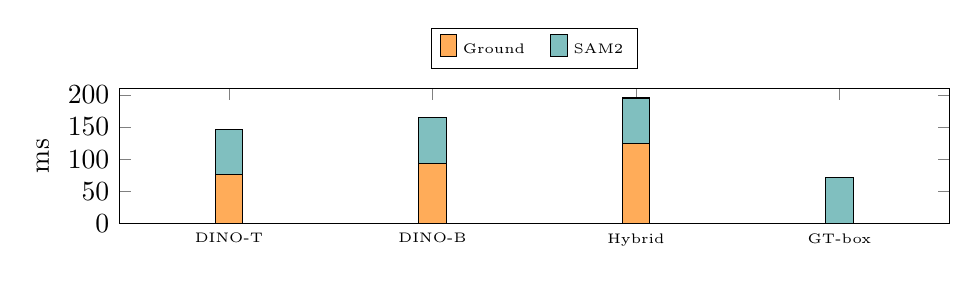
\begin{tikzpicture}
      \begin{axis}[
        width=\linewidth, height=3.3cm, ybar stacked, bar width=10pt,
        ymin=0, ymax=210, ylabel={ms},
        symbolic x coords={DINO-T,DINO-B,Hybrid,GT-box},
        xtick=data, xticklabel style={font=\tiny},
        legend style={
          font=\tiny,
          at={(0.5,1.14)},
          anchor=south,
          legend columns=2,
          /tikz/every even column/.append style={column sep=0.25cm}
        },
        enlarge x limits=0.18,
      ]
        \addplot[fill=orange!65] coordinates {(DINO-T,76) (DINO-B,94) (Hybrid,124) (GT-box,0)};
        \addplot[fill=teal!50] coordinates {(DINO-T,70) (DINO-B,71) (Hybrid,71) (GT-box,72)};
        \legend{Ground, SAM2}
      \end{axis}
    \end{tikzpicture}
    \par\vspace{0.15em}(d) RefCOCO latency breakdown
  \end{minipage}

  \vspace{0.55em}

  \begin{minipage}[t]{0.55\textwidth}
    \centering
    \begin{adjustbox}{max width=\linewidth}
    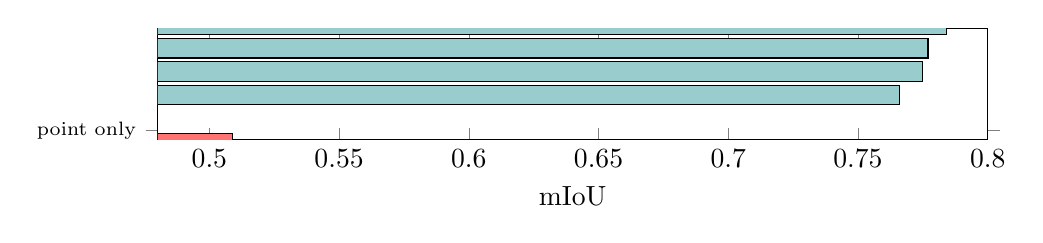
\begin{tikzpicture}
      \begin{axis}[
        width=\linewidth, height=3.0cm, xbar, bar width=7pt,
        xmin=0.48, xmax=0.80, xlabel={mIoU},
        symbolic y coords={point,boxpt,top1,default,full},
        yticklabels={point only, box+point, top1, default, no crop},
        ytick=data, yticklabel style={font=\scriptsize}, enlarge y limits=0.1,
      ]
        \addplot[fill=red!55] coordinates {(0.509,point)};
        \addplot[fill=teal!40] coordinates {(0.766,boxpt) (0.775,top1) (0.777,default) (0.784,full)};
      \end{axis}
    \end{tikzpicture}
    \end{adjustbox}
    \par\vspace{0.15em}(e) Adapter ablations
  \end{minipage}
  \caption{%
    \textbf{Quantitative summary.}
    (a) Hybrid is the best non-oracle method on RefCOCO, RefCOCO+, and RefCOCO-g.
    (b) Gains hold against both Grounding DINO baselines on every split.
    (c) Hybrid recovers 85.8--92.3\% of the GT-box oracle.
    (d) LocateAnything adds latency in exchange for stronger boxes.
    (e) Point-only prompting drops to $\sim$0.51 mIoU.}
  \label{fig:results-panel}
\end{figure*}
